\section{BACKGROUND}
\label{background}

\subsection{Notation}
\begin{itemize}
    \item $\mathcal{I}=\{O;\boldsymbol{X},\boldsymbol{Y},\boldsymbol{Z}\}$ denotes an inertial frame, composed of a point (origin) and an orientation as the ENU (East-North-Up) convention;% w.r.t.  the vehicle’s absolute pose is measured.

    \item $\mathcal{B}$ denotes the \emph{base frame}, i.e. a frame rigidly attached to the robot \emph{base link};
    
    \item $\mathcal{G}[\mathcal{I}]$ is a frame with the origin at the robot center of mass and the same orientation of the inertial frame;
    
    \item ${}^{\mathcal{I}}o_{\mathcal{G}} \in \mathbb{R}^3$ is the Center of Mass (CoM) position of the robot in the inertial frame. ${}^{\mathcal{I}}\boldsymbol{v}_{CoM} \in \mathbb{R}^3$ denotes the linear velocity of the robot CoM w.r.t. the inertial frame;

    \item ${}^{\mathcal{I}}\boldsymbol{v}_a \in \mathbb{R}^3$ indicates the relative velocity between the wind and the robot CoM expressed in the inertial frame, i.e. ${}^{\mathcal{I}}\boldsymbol{v}_a={}^{\mathcal{I}}\boldsymbol{v}_{CoM}-{}^{\mathcal{I}}\boldsymbol{v}_w$, with ${}^{\mathcal{I}}\boldsymbol{v}_w \in \mathbb{R}^3$ the absolute wind velocity\footnote{In the remainder of the paper, we omit the superscript $\mathcal{I}$ unless it is necessary to explicitly write it for the sake of clarity, and we write ${}^{\mathcal{I}}\boldsymbol{v}_a=\boldsymbol{v}_a$.};
    
    %\item $\mathcal{D}=\{{}^{\mathcal{I}}o_{\mathcal{G}};\boldsymbol{i},\boldsymbol{j},\boldsymbol{k}\}$ represents the \emph{body frame}.The $\boldsymbol{k}$ axis's direction lies along the line connecting the \emph{base frame} $\mathcal{B}$ origin and the origin of a frame attached to the robot head. The $\boldsymbol{j}$ axis's direction lies on the line that connects the origin of two frames attached to the right and left chest turbines. frame towards the origin of the left chest turbine frame on the plane that is perpendicular to the defined axis $\boldsymbol{k}$. The direction of $\boldsymbol{i}$ axis is defined by the right-hand rule;
    
    \item $\mathcal{D}=\{{}^{\mathcal{I}}o_{\mathcal{G}};\boldsymbol{i},\boldsymbol{j},\boldsymbol{k}\}$ represents the \emph{body frame}. The $\boldsymbol{k}$ axis direction is parallel to the chest cylinder principal axis, pointing towards the legs. The $\boldsymbol{j}$ axis is normal to the robot symmetry plane, pointing towards left arm. The $\boldsymbol{i}$ axis is defined by the right-hand rule;
    
    \item $\mathcal{A}=\{{}^{\mathcal{I}}o_{\mathcal{G}};\boldsymbol{X}_a,\boldsymbol{Y}_a,\boldsymbol{Z}_a\}$ is the \emph{relative velocity} frame, with the $\boldsymbol{Y}_a$ axis along the opposite direction of the relative velocity ${}^{\mathcal{I}}\boldsymbol{v}_a$.

    %\item $\boldsymbol{I}_n \in \mathbb{R}^{n \times n}$ is the identity matrix of size $n$; $0_{m \times n} \in \mathbb{R}^{m \times n}$ is the zero matrix of size $m\times n$ and $0_n=0_{n \times 1}$; 
    
    %\item $S(x) \in \mathbb{R}^{3 \times 3}$ is the skew-symmetric matrix such that $S(x)y=x \times y$, with $\times$ the cross product operator in $\mathbb{R}^3$;
    
\end{itemize}

\subsection{Robot Modeling}
The flying humanoid robot is modeled as a multi-body, \emph{floating-base} system composed of $n+1$ rigid bodies (\emph{links}). Each body is connected to the others by means of 1-DoF joints, for a total of $n$ DoF. The set of robot configurations belongs to a space defined as: $\mathbb{Q} \in \mathbb{R}^3 \times SO(3) \times \mathbb{R}^n$. The triplet $q=( {} ^{\mathcal{I}}o_{\mathcal{B}} , {} ^{\mathcal{I}}R_{\mathcal{B}} , s) \in \mathbb{Q}$ is composed of
%
\begin{figure}[t]
      \centering
      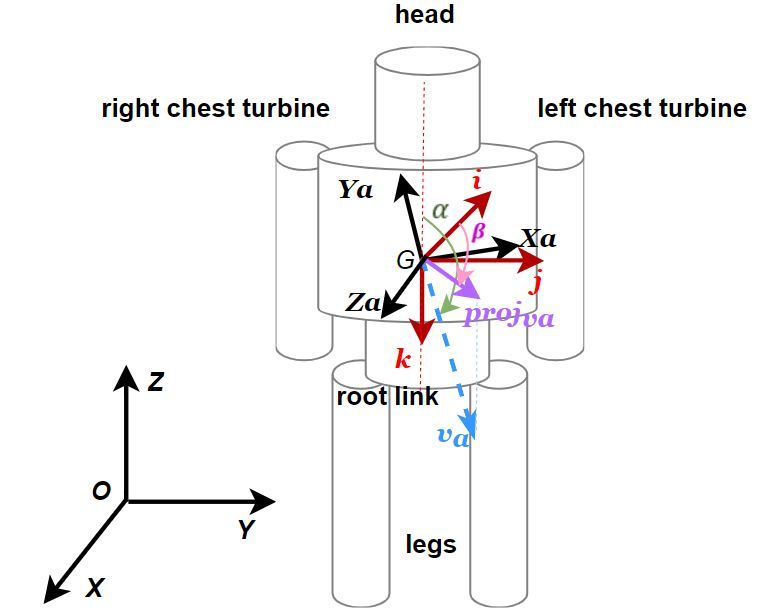
\includegraphics[width=80mm]{./imagines/frame_new01.jpg}
      \caption{Notation representation: inertial frame, body frame $\mathcal{D}$ (red color), relative velocity frame $\mathcal{A}$ (black color, on the robot), and $(\alpha,\beta)$ angles.} 
      \label{fig:notation} 
\end{figure}
%
$( {} ^{\mathcal{I}}o_{\mathcal{B}} , {} ^{\mathcal{I}}R_{\mathcal{B}})$, which represent the position and orientation of the base frame $\mathcal{B}$ w.r.t. the inertial frame, and the robot internal shape $s \in \mathbb{R}^n$ represented by the joint angles. The system velocities belong to the space $\mathbb{V} \in \mathbb{R}^3 \times \mathbb{R}^3 \times \mathbb{R}^n$. An element of $\mathbb{V}$ is given by $v=(v_{\mathcal{B}},\dot{s})$ where $v_{\mathcal{B}}=({}^{\mathcal{I}} \dot{o}_{\mathcal{B}},{}^{\mathcal{I}} \omega_{\mathcal{B}})$ is the linear and angular velocity of the base frame w.r.t. the inertial frame, while $\dot{s}$ are the joint velocities.

The floating-base system equations of motions can be derived following the Euler-Poincar$\acute{e}$ formalism \cite{c4}:
\begin{equation}
\label{eq_motion}
M(q)\dot{v}+C(q,v)v+G(q)=
\begin{bmatrix}
0_6\\
\tau
\end{bmatrix}
+\sum_{k=1}^{m}J_k^{\top} F_k ,
\end{equation}
where $M$, $C \in \mathbb{R}^{n+6\times n+6}$ are the mass and Coriolis matrix, $G \in \mathbb{R}^{n+6}$ is the gravity vector, $\tau \in \mathbb{R}^n$ are the internal actuation torques and $F_k$ is the $k^{th}$ external force acting on the system. In the case under study, we assume that the forces acting on the robot during flight are the aerodynamic forces and the thrust forces generated by the jet-engines. Here, we consider in the model only the thrust generated by the jet-engines, while the addition of aerodynamic forces in Eq.~(\ref{eq_motion}) will be treated later on in the paper. Hence, each $F_k \in \mathbb{R}^3$ represents the thrust force applied on the robot by the $k^{th}$ jet, and we rewrite $F_k={}^\mathcal{I}l_k T_k$, where ${}^\mathcal{I}l_k \in \mathbb{R}^3$ is the direction of thrust force, while $T_k \in \mathbb{R}$ is the thrust intensity. The jacobian $J_k(q)$ is the map between the system velocity $v$ and the linear velocity ${}^\mathcal{I} \dot{o}_k$ of the $k^{th}$ thrust application point. We can then define the thrusts vector $T:=(T_1, T_2, T_3, T_4)^{\top}$ and rewrite $\sum^{m}_{k=1}J_k^{\top}F_k = f(q,T)$.


\subsection{Modeling of Aerodynamic Forces}
\label{sec:af}
% The aerodynamic forces acting on the robot during flight can be modeled in different ways. For example, one could: 1) consider separately the aerodynamic forces acting at the Center of Pressure (CoP) of each robot link; or, 2) evaluate the \emph{total} aerodynamic force acting on the robot, i.e., the sum of all forces on the bodies composing the robot. We chose to follow the second route, because the simplified geometry of the robot model we used for CFD analysis allows to achieve more reliable results when looking at the global forces acting on the system, while the geometry approximation has a bigger impact in calculating the correct forces locally on each single body.
%\tongsays{due to the less of pages, this part may be shorten a bit, Tong is working on it}
 We prefer to model the \emph{global} aerodynamic force acting on the robot, because evaluating aerodynamic effects distributed on several parts of the body requires to design a more complex robot model for the CFD analysis, which becomes very time consuming. The global aerodynamic effects at the robot CoM are composed of the aerodynamic force ${F}_a \in \mathbb{R}^3$, and the moment ${M}_a:={\mathcal{G}P}\times {F}_a \in \mathbb{R}^3$, where ${\mathcal{G}P}$ is the distance between the CoM $\mathcal{G}$ and the Center of Pressure (CoP) $P$. 

Consider any pair of angles $(\alpha, \beta)$ characterizing the relative orientation of $\boldsymbol{v}_a$ w.r.t. the body frame $\mathcal{D}$, chosen as in  Fig.~\ref{fig:notation}. $\alpha \in [0,\pi]$ is defined as the angle between $\boldsymbol{v}_a$ and the negative $\boldsymbol{k}$ axis of the body frame $\mathcal{D}$, while $\beta \in [0,2\pi]$ is defined as the angle between the projection of $\boldsymbol{v}_a$ on plane $(\boldsymbol{i},\boldsymbol{j})$ and the positive $\boldsymbol{i}$ axis of frame $\mathcal{D}$ (see also \cite{c3}).

The aerodynamic force can be decomposed w.r.t. the relative velocity frame $\mathcal{A}$ as:
\begin{equation}
\label{eq:af_total_control}
{F}_a={F}_D+{F}_S+{F}_N ,
\end{equation}
where:
\begin{itemize}
    \item ${F}_D$, the drag force, aligns with $\boldsymbol{Y}_a$ axis;
    \item ${F}_S$, the defined sideforce, aligns with $\boldsymbol{X}_a$ axis;
    \item ${F}_N$, the defined normal force, aligns with $\boldsymbol{Z}_a$ axis.
\end{itemize}
The intensity of the steady aerodynamic force varies approximately with $|\boldsymbol{v}_a|^2$, hence there exist three dimensionless functions $C_D$, $C_S$, $C_N$ depending on the Reynolds number $Re$, the Mach number $\mathcal{M}$ and $(\alpha, \beta)$, such that \cite{c3}\cite{c5}:
\begin{subequations}
\begin{align}
    {F}_D & :=\mathcal{K}_a|\boldsymbol{v}_a|^2C_D(Re, \mathcal{M}, \alpha, \beta)\boldsymbol{j}_a,\\
    {F}_S & :=\mathcal{K}_a|\boldsymbol{v}_a|^2C_S(Re, \mathcal{M}, \alpha, \beta)\boldsymbol{i}_a,\\
    {F}_N & :=\mathcal{K}_a|\boldsymbol{v}_a|^2C_N(Re, \mathcal{M}, \alpha, \beta)\boldsymbol{k}_a,
\end{align}
\label{eq:af_coe}
\end{subequations}
 where $\mathcal{K}_a:=\frac{A_{ref}\rho}{2}$ with $\rho$ the air density and $A_{ref}$ the reference frontal area;  $\boldsymbol{i}_a$, $\boldsymbol{j}_a$, $\boldsymbol{k}_a$ are the unit vectors of frame $\mathcal{A}$ along $\boldsymbol{X}_a$, $\boldsymbol{Y}_a$, $\boldsymbol{Z}_a$ axes.
In particular, $\boldsymbol{j}_a$ has the opposite direction of $\boldsymbol{v}_a$ by definition. Identifying the numerical relation among the dimensionless coefficients $C_D$, $C_S$, $C_N$ and their variables is fundamental for the design of analytical models of the aerodynamic forces to be in the system modeling and control design. 

